\documentclass{article}

\usepackage{Engineering}
\pdftitle{Electrical-eng}

% === TEXT ===
\title{\textbf{Electrical Engineering \\ HSLU, Semester 2}}
\author{Matteo Frongillo}
\date{}

\begin{document}

\maketitle
\tableofcontents
\pagebreak

\part{...}
\section{...}
\subsection{Current strength or current ``I''}
\begin{center}
    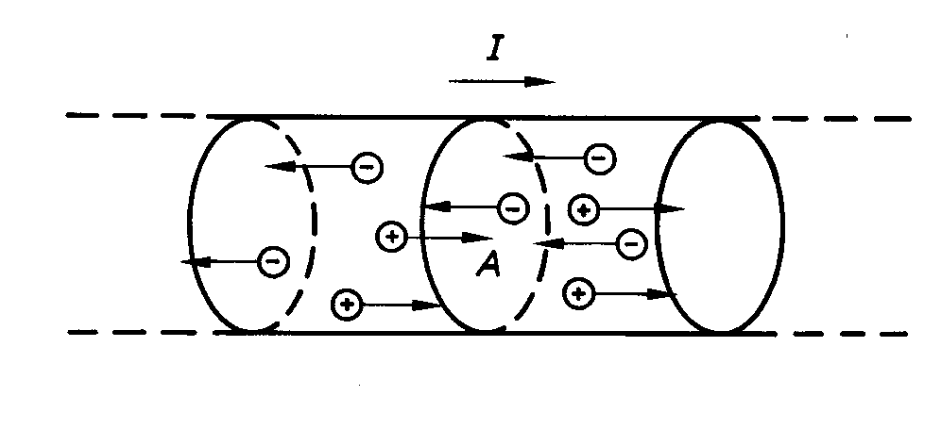
\includegraphics[width=.4\textwidth]{media/intensity.png}
\end{center}
\[I\ [A] =\dfrac{\text{el. charge}}{t}\]

\subsection{Current density ``J''}
\begin{center}
    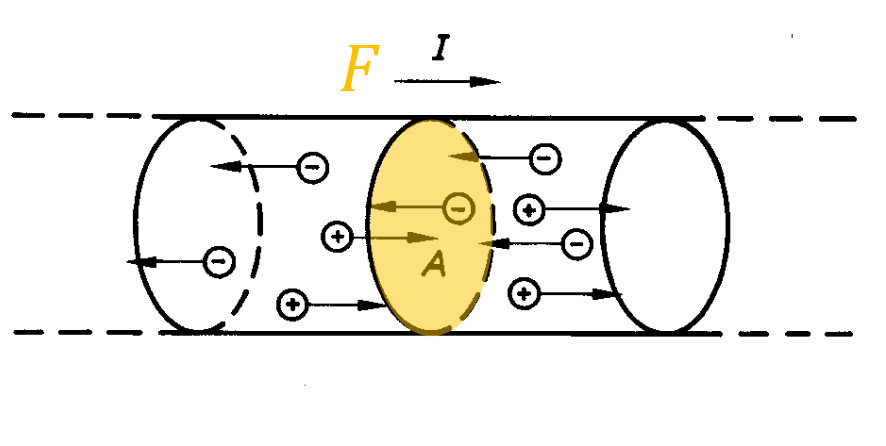
\includegraphics[width=.4\textwidth]{media/density.png}
\end{center}
The current density indicates how large the current per cross-sectional area (F) is:
\[J\ [\dfrac{A}{mm^2}] = \dfrac{I}{F}\]

\subsection{Temperature dependence of the resistance}
\begin{center}
    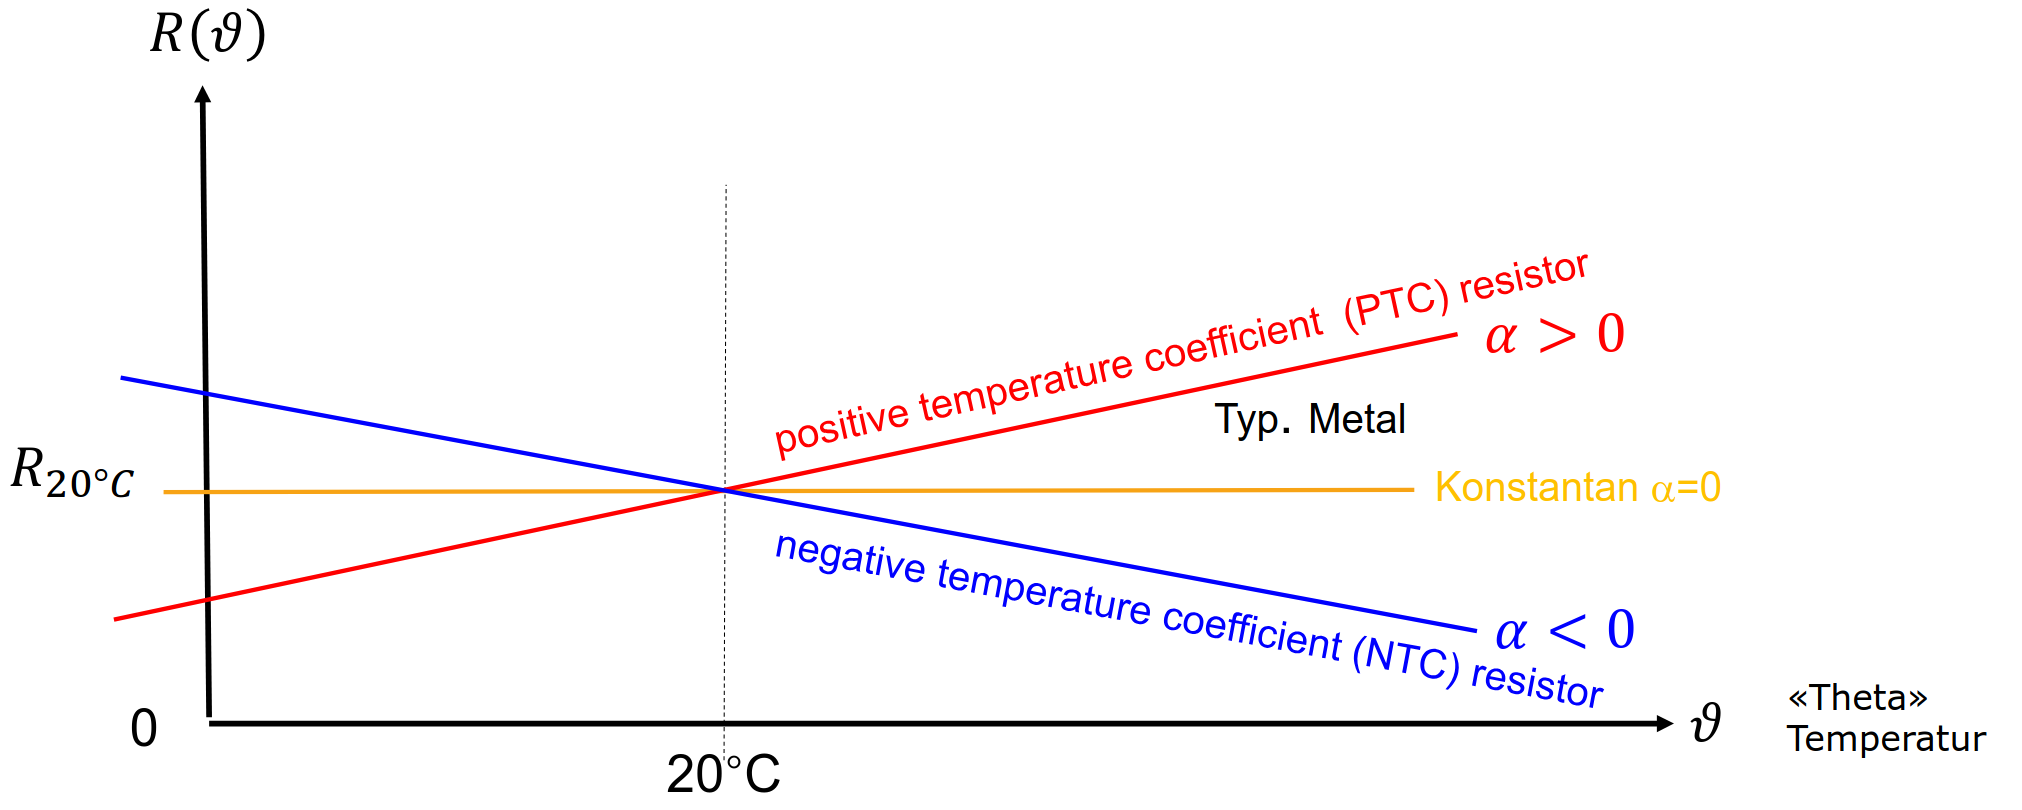
\includegraphics[width=\textwidth]{media/resistance.png}
\end{center}
Depending on the material, the resistance can increase, remain the same or decrease with temperature. In
ET+L we calculate using the linear approach.
\figbox{$R(\vartheta) = R_{20}(1+\alpha(\vartheta-20^{\circ}\text{C})) = R_{20}(1+\alpha \Delta T)$}

\subsection{Object properties}
The resistance indicates the voltage required for a
current. In addition to the material, the cross-sectional
area and also the length are decisive factors.
\[R=\frac{U}{I}\]

\subsection{Reciprocal quantities}
\subsubsection{Specific resistance}
To describe material properties, the resistance per length
and cross-sectional area is specified (precondition:
homogeneous conductor, direct current):
\[\rho\ [\frac{\Omega \cdot mm^2}{m}] = R\cdot \frac{A}{l}\]

\subsubsection{Conductance}


\subsubsection{Specific conductivity}

\newpage
\section{Gravitational fields}
\subsection{Between bodies}
\efigbox{F_1 = F_2 = G\dfrac{m_1m_2}{d^2}}

\subsection{Between particles}
\subsubsection{Coulomb's law}
It calculates the amount of force between two electrically charged
particles at rest:
\efigbox{F=\dfrac{1}{4\pi \varepsilon_0} \cdot \dfrac{q_1q_2}{r^2}}

where:
\begin{itemize}
    \item $F$: Force [N];
    \item $q$: Charge [As];
    \item $\varepsilon_0$: absolute permittivity = $8.8542\cdot 10^{-12}$ [As/Vm].
\end{itemize}

\subsection{Electric field and force on a charge $Q$}
\subsubsection{Homogeneous electric fields}
\efigbox{E=\dfrac{U}{d}}

where:
\begin{itemize}
    \item $E$: electric field strength [V/m];
    \item $U$: voltage [V];
    \item $d$: distance of the electrodes [m].
\end{itemize}

\subsubsection{Force on a point charge}
\efigbox{F=Q\cdot E}

where:
\begin{itemize}
    \item $E$: electric field strength [V/m];
    \item $Q$: charge [As];
    \item $F$: force [N].
\end{itemize}

\newpage
\section{Capacitance and Capacitor}
\subsection{Capacitor}
A capacitor is a device in which the capacitance is used.

\subsection{Capacitance}
Capacitance $C$ is the \textbf{capability} to store electric charge.
It is measured by the charge divided by the applied voltage:
\efigbox{C=\dfrac{Q}{U}}

where:
\begin{itemize}
    \item $Q$: charge [As];
    \item $U$: voltage [V];
    \item $C$: capacitance [As/V = F (Farad)].
\end{itemize}

\subsubsection{Capacitance of a plate capacitor}
\efigbox{C=\varepsilon\cdot \dfrac{A}{d}}

where:
\begin{itemize}
    \item $A$: plate area (one side) [m$^2$];
    \item $d$: distance between plates [m];
    \item $C$: capacitance [F].
\end{itemize}

\pph{Permittivity}
\efigbox{\varepsilon = \varepsilon_r\cdot \varepsilon_0}
\begin{itemize}
    \item $\varepsilon_r$: relative permittivity of the dielectric, relative to the air;
    \item $\varepsilon_0$: absolute permittivity [As/Vm].
\end{itemize}

\subsubsection{Energy in a capacitor}
If a capacitor is discharged with a constant current, the voltage decreases linearly:

\efigbox{\int_{0}^{t_{\text{empty}}}U(t)\cdot I\,dt = I\cdot U_0 = \frac{I\cdot U_0 \cdot t_{\text{empty}}}{2}}

Or, simplified:
\efigbox{W=\frac{1}{2}C\cdot U_0^2}

where:
\begin{itemize}
    \item $W$: energy [J or Ws];
    \item $U_0$: initial voltage [V];
    \item $C$: capacitance [F].
\end{itemize}

\subsection{Capacitors in parallel connection}
Capacitances connected in parallel add up:
\efigbox{C_{\text{tot}} = \frac{\sum_{n} Q_n}{U} = \sum_{n} C_n}

or

\efigbox{C = \frac{\varepsilon\cdot \left(\sum_{n} A_n\right)}{d} = \sum_{n} C_n}

\subsection{Capacitors in series connection}
In a series connection, the reciprocal of the total capacitance is the sum of the reciprocals of the individual capacitances:
\efigbox{\frac{1}{C_{\text{tot}}} = \sum_{n}\frac{1}{C_n}}

where:
\begin{itemize}
    \item $C_{\text{tot}}$: total capacitance [F];
    \item $C_n$: capacitance of the $n$-th capacitor [F].
\end{itemize}

\section{Transient Analysis in RC Circuits}
\subsection{Charging of a Capacitor}
When a capacitor is charged through a resistor, the voltage across it increases exponentially:
\efigbox{U_C(t)= U_0\cdot\left(1-e^{-t/(R\cdot C)}\right)}

with the time constant defined as:
\efigbox{\tau=R\cdot C}

where:
\begin{itemize}
    \item $U_C(t)$: voltage across the capacitor at time $t$ [V];
    \item $U_0$: applied voltage [V];
    \item $R$: resistance [$\Omega$];
    \item $C$: capacitance [F];
    \item $\tau$: time constant [s].
\end{itemize}

\subsection{Discharging of a Capacitor}
When a charged capacitor discharges through a resistor, the voltage decays exponentially:
\efigbox{U_C(t)= U_0\cdot e^{-t/(R\cdot C)}}

and the discharging current is:
\efigbox{I(t)= \frac{U_0}{R}\cdot e^{-\frac{t}{(R\cdot C)}}}

\newpage
\subsection{Transitional phase}
\efigbox{f(t)=A+\Delta\cdot \left(1-e^{t/\tau}\right) = A+(B-A)\cdot (1-e^{1/\tau})}

\section{Additional Topics}
\subsection{Energy Stored in a Capacitor}
The energy stored in a capacitor is given by:
\efigbox{W=\frac{1}{2}C\cdot U_0^2}

where:
\begin{itemize}
    \item $W$: energy [J];
    \item $C$: capacitance [F];
    \item $U_0$: voltage [V].
\end{itemize}

\subsection{Charge--Voltage Relationship}
For an ideal capacitor, the relationship between charge and voltage is:
\efigbox{Q=C\cdot U}

Moreover, the current is the time derivative of the charge:
\efigbox{I=\frac{dQ}{dt}=C\cdot\frac{dU}{dt}}

Note that the voltage across an ideal capacitor cannot change instantaneously.

\newpage

\end{document}
